\newpage
\section{Introduction}
\label{sec:introduction}

%state the learning objective 
The objective of this laboratory assignment is to build a bandpass filter with a central frequency of 1kHz and a gain of 40dB.
The circuit created and analysed in this assignment can be seen in Figure~\ref{fig:Circuit}.\\
\noindent In order to evaluate how successfully our goal has been achieved, we calculate the merit M of our work, using the following expression:
\begin{equation}
M = \frac{1}{cost(*GainDeviation*CentralFreqDeviation + 10^{-6})}
  \label{eq:merit}
\end{equation}
where the cost is given by cost = cost of resistors + cost of capacitors + cost of transistors, knowing that each kOhm costs 1 monetary unit (MU), 
each $\mu$F costs 1 MU and each transistor costs 0,1 MU.
\noindent In Section~\ref{sec:analysis}, a theoretical analysis of the circuit is
presented, using Octave. In Section~\ref{sec:simulation}, the circuit is analysed by
simulation using ngspice. The conclusions of this study are outlined in
Section~\ref{sec:conclusion}. In addiction, the results are compared to the theoretical results obtained in Section~\ref{sec:analysis}.

\begin{figure}[h!] \centering
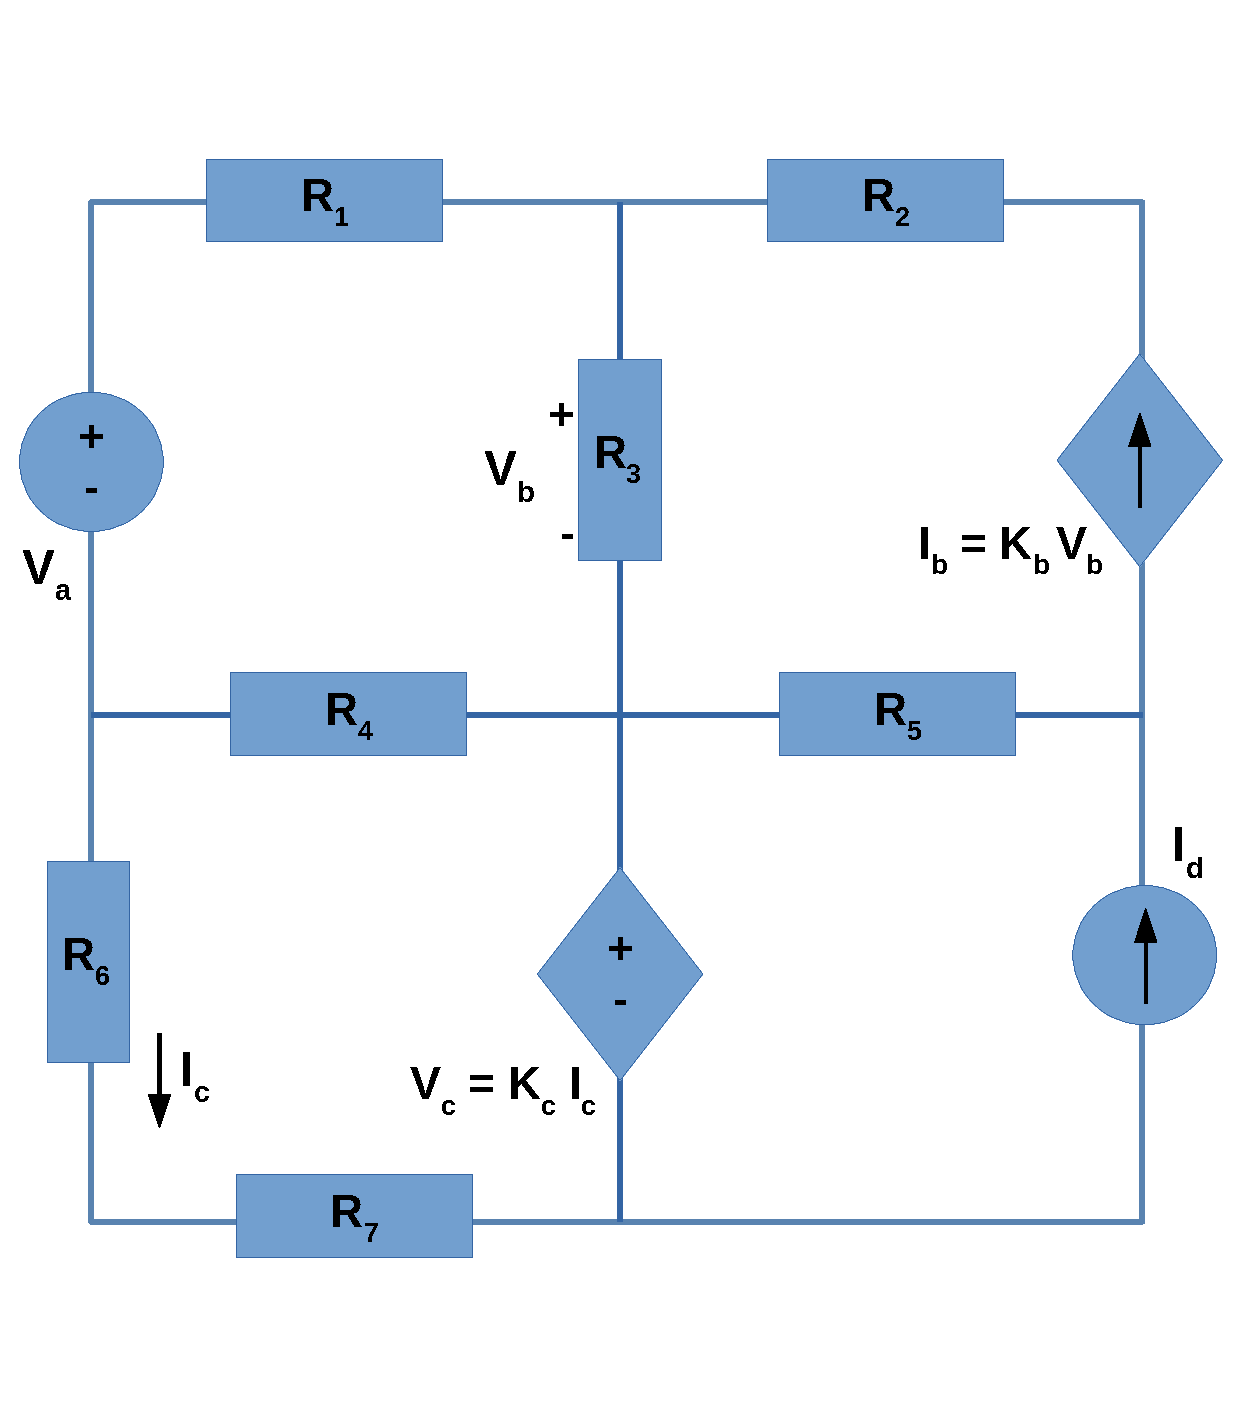
\includegraphics[width=1\linewidth]{Circuit.pdf}
\caption{Circuit analysed.}
\label{fig:Circuit}
\end{figure}

